\documentclass[aspectratio=169,10pt]{beamer}

\usepackage{booktabs}
\usepackage{graphicx}
\usepackage{amsmath}
\usepackage{xcolor}

\usetheme{Madrid}
\usecolortheme{seahorse}
\setbeamertemplate{navigation symbols}{}
\setbeamertemplate{caption}[numbered]
\setbeamerfont{title}{size=\LARGE,series=\bfseries}
\setbeamerfont{frametitle}{size=\large,series=\bfseries}
\setbeamertemplate{itemize items}[circle]
\setlength{\parskip}{2pt}

\title{When does A* save work?}
\subtitle{T01: structure, heuristic and the cost of guidance}
\author[E. Haqqverdiyev, R. Iskandarli]{Elnur Haqqverdiyev \and Rajab Iskandarli}
\institute[UFAZ]{UFAZ, M1 Data Science and AI\\Advanced Data Structures and Algorithms, Fall 2026}
\date{Defence}

\begin{document}

\begin{frame}
  \titlepage
\end{frame}

\begin{frame}{The question}
  \begin{columns}[T,onlytextwidth]
    \begin{column}{0.52\textwidth}
      \textbf{Dijkstra} expands every vertex closer than the target.\\
      \textbf{A*} adds a heuristic $h(v)$ and expands fewer vertices.
      \vspace{0.5em}

      \textbf{But guidance is not free:}
      \begin{itemize}
        \item one heuristic evaluation per generated vertex;
        \item larger heap keys / more memory traffic;
        \item a weak heuristic can save nothing.
      \end{itemize}
    \end{column}
    \begin{column}{0.44\textwidth}
      \begin{block}{Research question}
        How do graph structure and heuristic strength change
        \begin{itemize}
          \item expanded vertices and
          \item wall-clock runtime
        \end{itemize}
        of A* versus Dijkstra, on unit-cost grids and a real road graph?
      \end{block}
    \end{column}
  \end{columns}
  \vspace{0.6em}
  \centering
  \large The answer must separate \textbf{expansions} from \textbf{time}.
\end{frame}

\begin{frame}{Data: synthetic controls and a real graph}
  \begin{columns}[T,onlytextwidth]
    \begin{column}{0.47\textwidth}
      \textbf{Grids} --- 4-neighbour, unit cost, 128--1024 square
      \begin{itemize}
        \item open
        \item random 20\% obstacles
        \item clustered 30\% obstacles
        \item rooms (walls with doors)
        \item perfect maze
      \end{itemize}
      \small Largest 4-connected component is used. Blocked cells are isolated
      vertices.
    \end{column}
    \begin{column}{0.50\textwidth}
      \textbf{Real graph: SNAP \texttt{roadNet-CA}}
      \begin{itemize}
        \item California road network
        \item 1,957,027 vertices after symmetrisation and largest component
        \item 2,760,388 undirected edges (5,520,776 CSR arcs)
        \item unit hop weight: SNAP has no lengths/travel times
      \end{itemize}
      \vspace{0.3em}
      \small One sparse, planar-like road graph; one limitation, not a sample
      of all real graphs.
    \end{column}
  \end{columns}
  \vspace{0.7em}
  \centering
  \begin{tabular}{lcc}
    \toprule
    experiment & query instances & timed runs\\
    \midrule
    grids (20 graphs) & 300 & 2,700\\
    real graph & 30 & 900\\
    \midrule
    total & 330 & 3,600\\
    \bottomrule
  \end{tabular}
\end{frame}

\begin{frame}{What we built: ADTs and complexity}
  \begin{columns}[T,onlytextwidth]
    \begin{column}{0.49\textwidth}
      \begin{block}{Graph: CSR}
        \small
        \texttt{offsets[n+1]}, \texttt{targets[m]}, \texttt{weights[m]}\\
        memory $O(n+m)$; neighbour iteration $O(\deg u)$
      \end{block}
      \begin{block}{Binary heap}
        \small
        push/pop $O(\log n)$ worst case; top $O(1)$\\
        lazy deletion: no decrease-key; stale entries are detected on pop\\
        ties: \texttt{node\_id} vs \texttt{larger\_g}
      \end{block}
    \end{column}
    \begin{column}{0.49\textwidth}
      \begin{block}{One search loop}
        \small
        Dijkstra = same loop with $h\equiv 0$\\
        A* $= f=g+h(v)$; stop when target is settled\\
        consistent heuristic $\Rightarrow$ no reopening\\
        scratch arrays reset in $O(1)$ by generation stamp
      \end{block}
      \begin{block}{Heuristics}
        \small
        grids: Manhattan (admissible + consistent)\\
        road: ALT $\max_L |d(L,v)-d(L,t)|$\\
        16 landmarks by farthest-point sampling; main $K=8$
      \end{block}
    \end{column}
  \end{columns}
\end{frame}

\begin{frame}{Correctness first}
  \begin{columns}[T,onlytextwidth]
    \begin{column}{0.52\textwidth}
      \textbf{Tests before any timing}
      \begin{itemize}
        \item heap order vs reference priority queue
        \item hand-computed 5x5 wall grid: distance 8
        \item hand-computed weighted graph vs Floyd--Warshall
        \item all five grid families vs independent BFS
        \item ALT admissibility and consistency for every free vertex
        \item path validation: contiguous edges, weights sum to distance
      \end{itemize}
    \end{column}
    \begin{column}{0.45\textwidth}
      \begin{block}{Oracle and audit}
        Every benchmark query is checked against BFS distance.
        \vspace{0.3em}

        \textbf{3,600 / 3,600} runs: \texttt{status=ok}, distance matches
        oracle, zero timeouts.\\
        \vspace{0.3em}
        Expansions deterministic across repeats; median time CV $\approx$ 7--10\%.
      \end{block}
    \end{column}
  \end{columns}
  \vspace{0.6em}
  \centering
  \small
  \begin{tabular}{ll}
    \toprule
    counter & definition (short)\\
    \midrule
    expanded & popped, not stale, not closed; target included\\
    pushed & source + every successful distance decrease\\
    stale\_popped & old heap entry or already-closed vertex\\
    time\_ns & search call only; inputs outside timer\\
    \bottomrule
  \end{tabular}
\end{frame}

\begin{frame}{Frozen protocol}
  \begin{columns}[T,onlytextwidth]
    \begin{column}{0.51\textwidth}
      \begin{itemize}
        \item paired Dijkstra/A* on exactly the same query
        \item 15 grid queries/graph, 30 real queries
        \item 3 grid repeats, 5 real repeats
        \item one untimed warm-up per treatment
        \item report median per query; keep raw repeats
        \item bootstrap 95\% CI + paired Wilcoxon
        \item 30 s cap per search; 4 GiB process cap
        \item one CPU via \texttt{taskset}
      \end{itemize}
    \end{column}
    \begin{column}{0.46\textwidth}
      \begin{block}{Query bands}
        \small
        BFS distance from a random source:
        \begin{itemize}
          \item short: 8--25\% of eccentricity
          \item medium: 40--60\%
          \item long: 80--97\%
        \end{itemize}
        Selection uses only BFS, never Dijkstra/A*.
      \end{block}
      \begin{block}{Freeze}
        Predictions in \texttt{HYPOTHESES.md}; protocol fixed before the main
        run in \texttt{PROTOCOL.md}.
      \end{block}
    \end{column}
  \end{columns}
\end{frame}

\begin{frame}{Predictions before the main run}
  \small
  \setlength{\tabcolsep}{4pt}
  \begin{tabular}{p{0.05\textwidth}p{0.78\textwidth}p{0.11\textwidth}}
    \toprule
    & prediction & verdict\\
    \midrule
    H1 & open grid: A* saves many expansions and time & confirmed\\
    H2 & random obstacles: still saves, less than open & confirmed\\
    H3 & clustered/rooms: weaker than open; rooms weaker than random & confirmed\\
    H4 & maze: no expansion saving; A* slower & confirmed\\
    H5 & long queries benefit more than short & partly rejected\\
    H6 & ALT strong at K=8; K=1 may not help; diminishing at 16 & partly rejected\\
    H7 & \texttt{larger\_g} reduces median expansions on open & rejected as median claim\\
    \bottomrule
  \end{tabular}
  \vspace{0.7em}

  The protocol explicitly allowed negative and null results.
\end{frame}

\begin{frame}{Main grid result}
  \centering
  \small
  \begin{tabular}{lcccc}
    \toprule
    family & time ratio & expansion ratio & time saving & A* faster\\
           & (median) & (median) & (median) & queries\\
    \midrule
    open          & \textbf{105.7x} & \textbf{222.4x} & 99.1\% & 100\%\\
    random 20\%   & 12.8x & 21.4x & 92.2\% & 98\%\\
    clustered 30\%& 12.8x & 22.9x & 92.2\% & 98\%\\
    rooms         & 8.7x  & 14.3x & 88.5\% & 100\%\\
    maze          & \textbf{0.81x} & \textbf{1.02x} & \textbf{--24.0\%} & 17\%\\
    \bottomrule
  \end{tabular}
  \vspace{0.15em}

  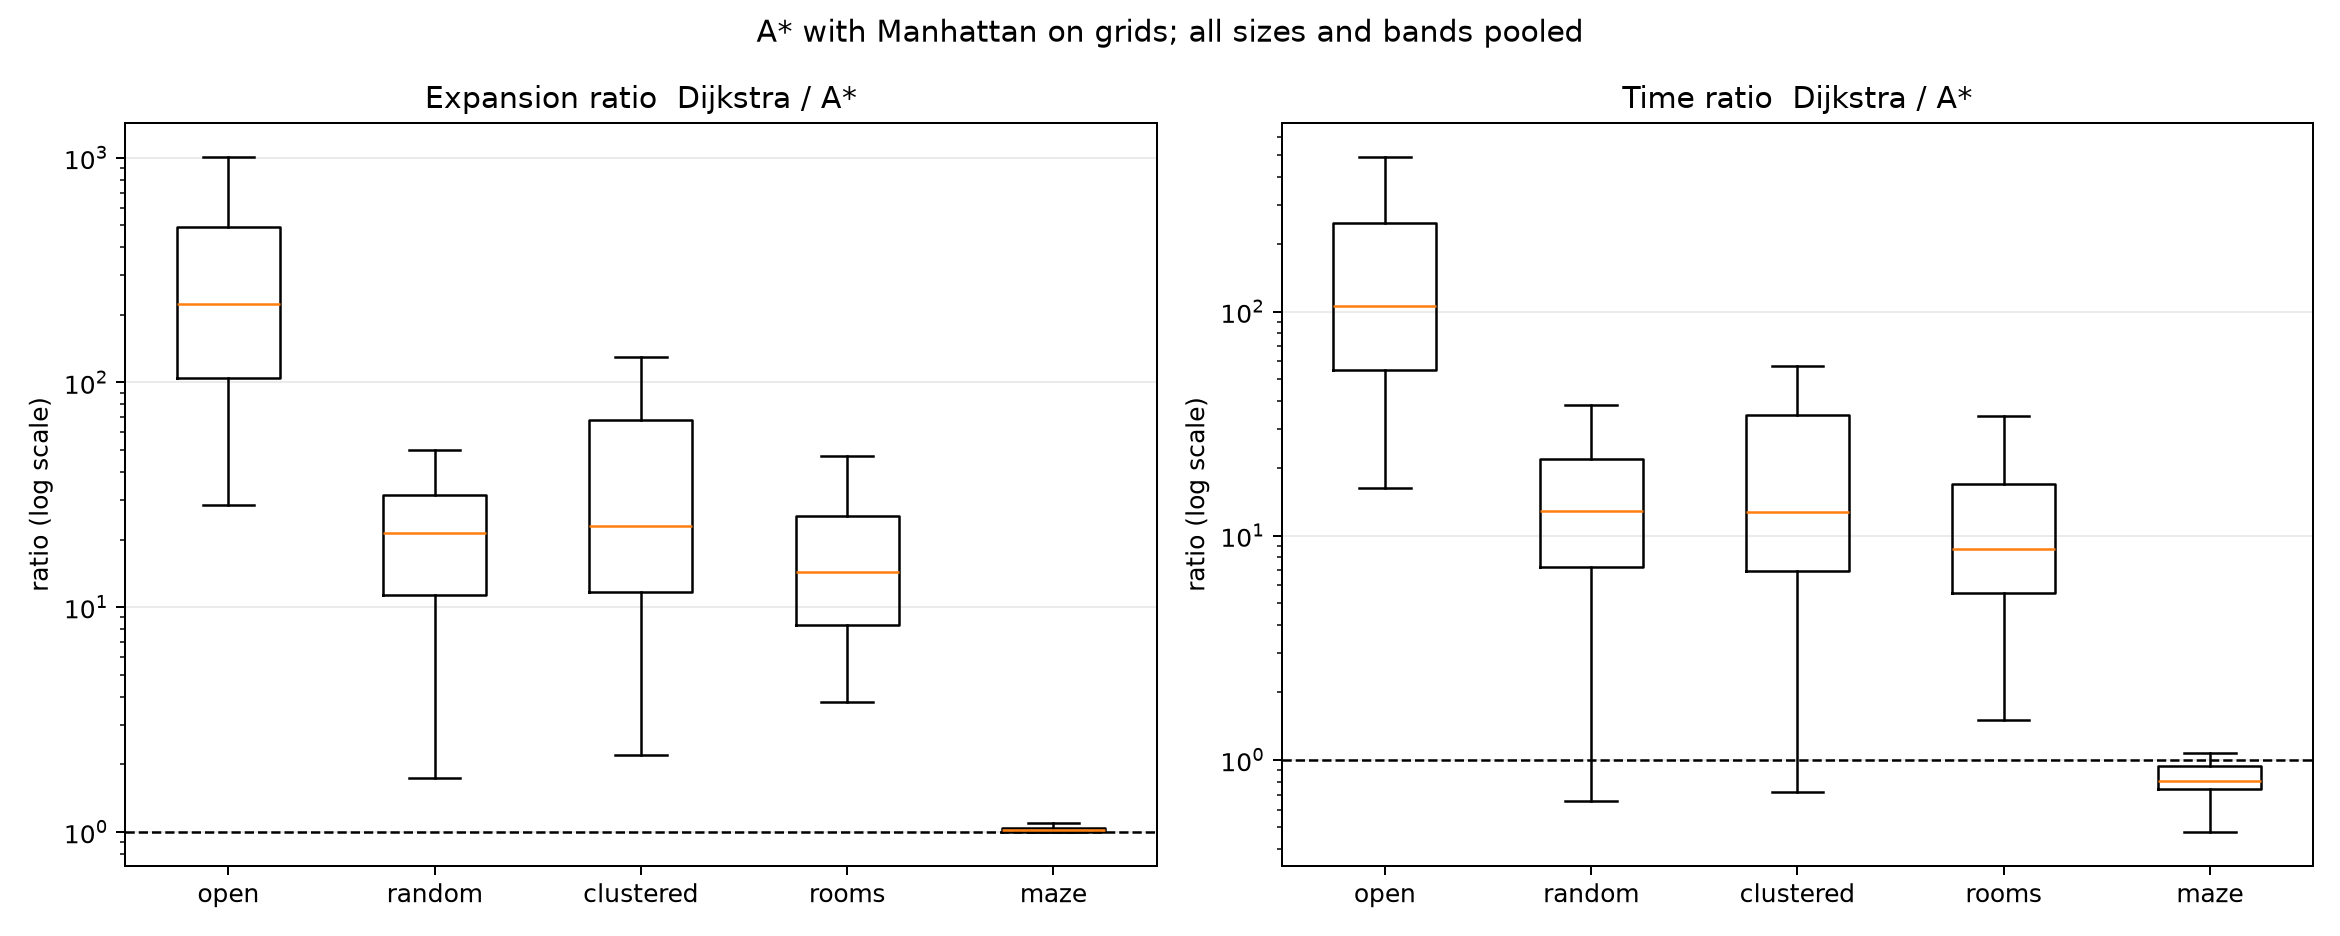
\includegraphics[width=0.63\textwidth]{../figures/grid_ratios_by_family.png}

  \footnotesize Ratio = Dijkstra / A*; values above 1 mean A* wins.
\end{frame}

\begin{frame}{Structure matters more than distance}
  \begin{columns}[T,onlytextwidth]
    \begin{column}{0.50\textwidth}
      \centering
      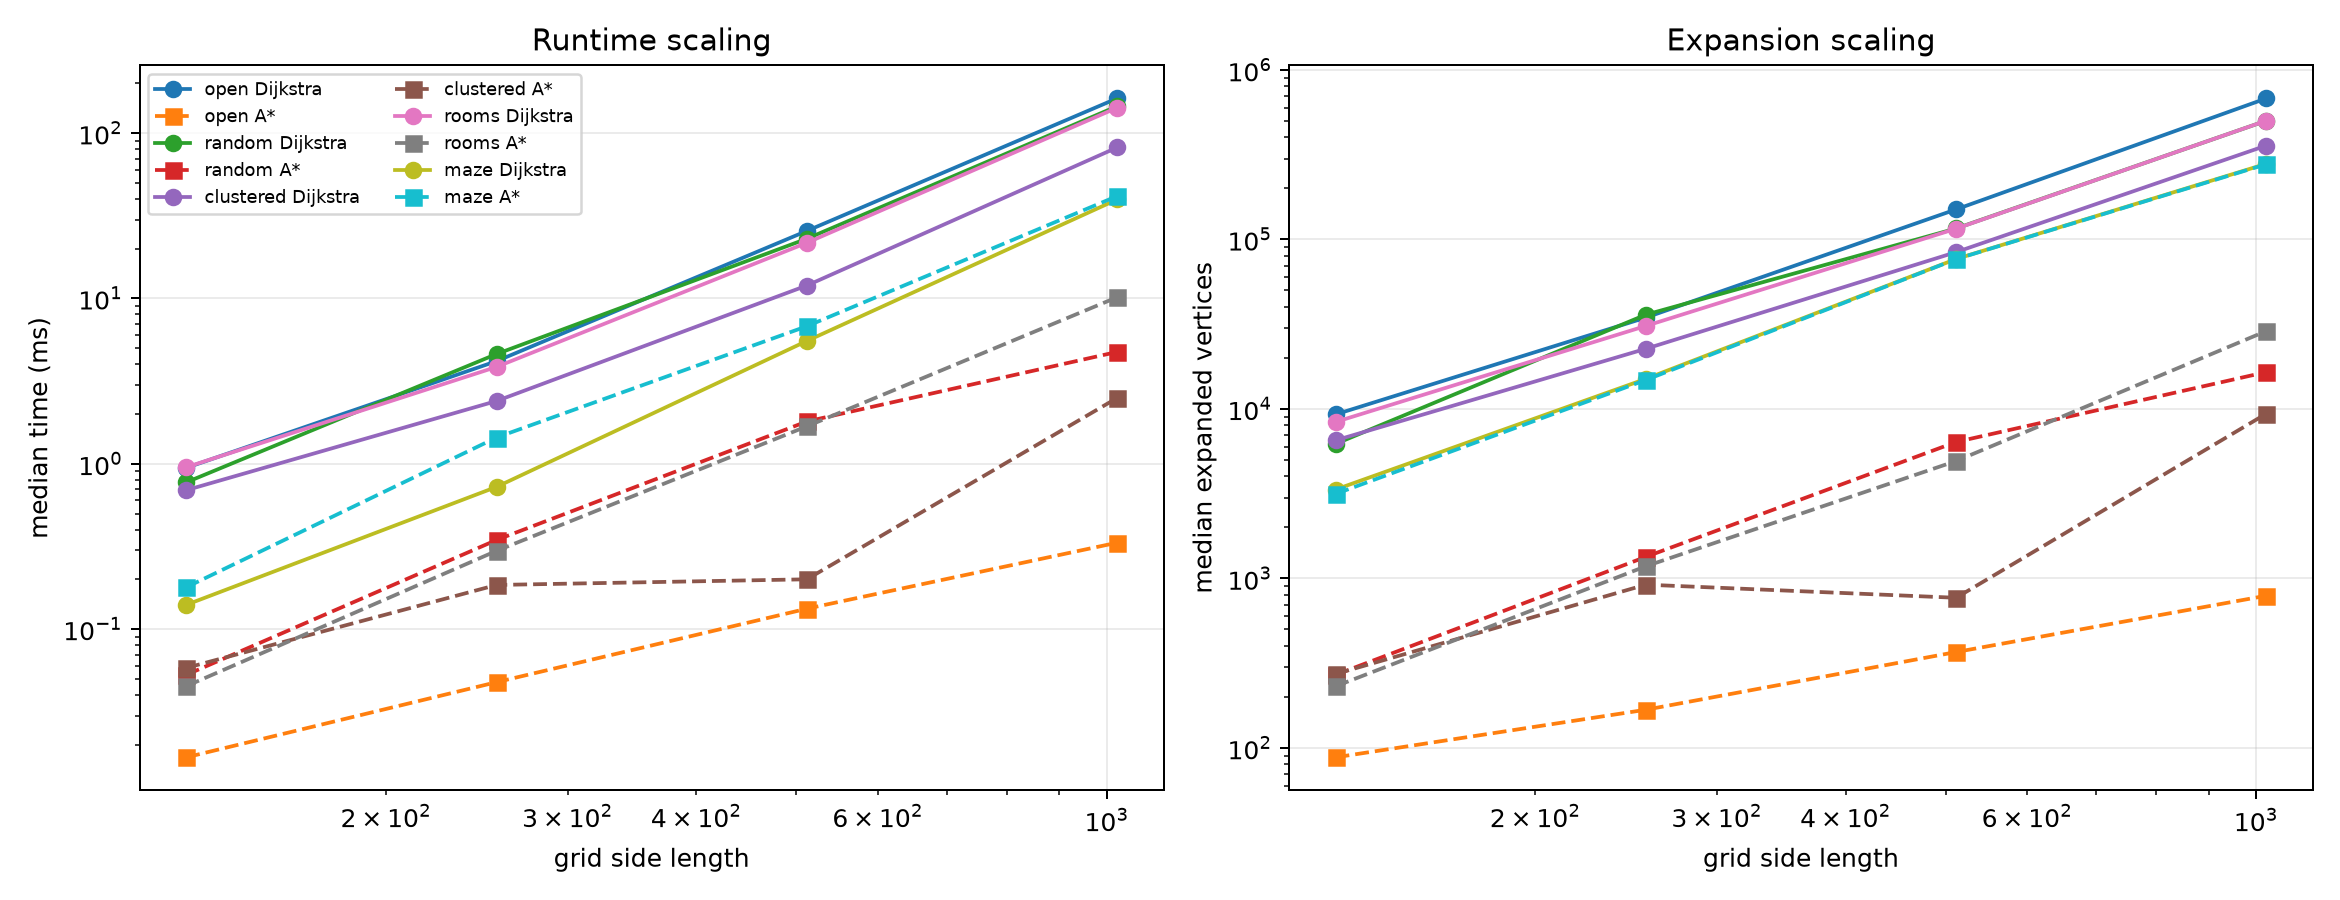
\includegraphics[width=\textwidth]{../figures/grid_scaling.png}
    \end{column}
    \begin{column}{0.47\textwidth}
      \textbf{Open grid:} A* follows one corridor; the advantage grows with
      size (390x time, 696x expansions at 1024).
      \vspace{0.5em}

      \textbf{Random/clustered:} local detours cost some guidance power; still
      8--13x time.
      \vspace{0.5em}

      \textbf{Rooms:} long forced detours; weakest positive family (8.7x).
      \vspace{0.5em}

      \textbf{Maze:} Manhattan cannot see the forced turns.  A* is
      \textbf{24\% slower}; expansions are essentially unchanged.
    \end{column}
  \end{columns}
\end{frame}

\begin{frame}{Real road network: ALT makes A* worthwhile}
  \begin{columns}[T,onlytextwidth]
    \begin{column}{0.55\textwidth}
      \centering
      \small
      \begin{tabular}{lcccc}
        \toprule
        ALT & time ratio & exp.\ ratio & time saving & faster\\
        \midrule
        K=1  & 1.29x & 1.96x & 22.5\% & 70\%\\
        K=4  & 4.75x & 7.26x & 78.9\% & 100\%\\
        K=8  & \textbf{7.62x} & \textbf{11.54x} & 86.8\% & 100\%\\
        K=16 & \textbf{13.52x} & \textbf{22.41x} & 92.6\% & 100\%\\
        \bottomrule
      \end{tabular}

      \vspace{0.4em}
      \footnotesize K=1 time difference not significant (p=0.13); K=4/8/16
      p$<$1e-8. K=16 is 21\% faster than K=8 on paired queries.
    \end{column}
    \begin{column}{0.43\textwidth}
      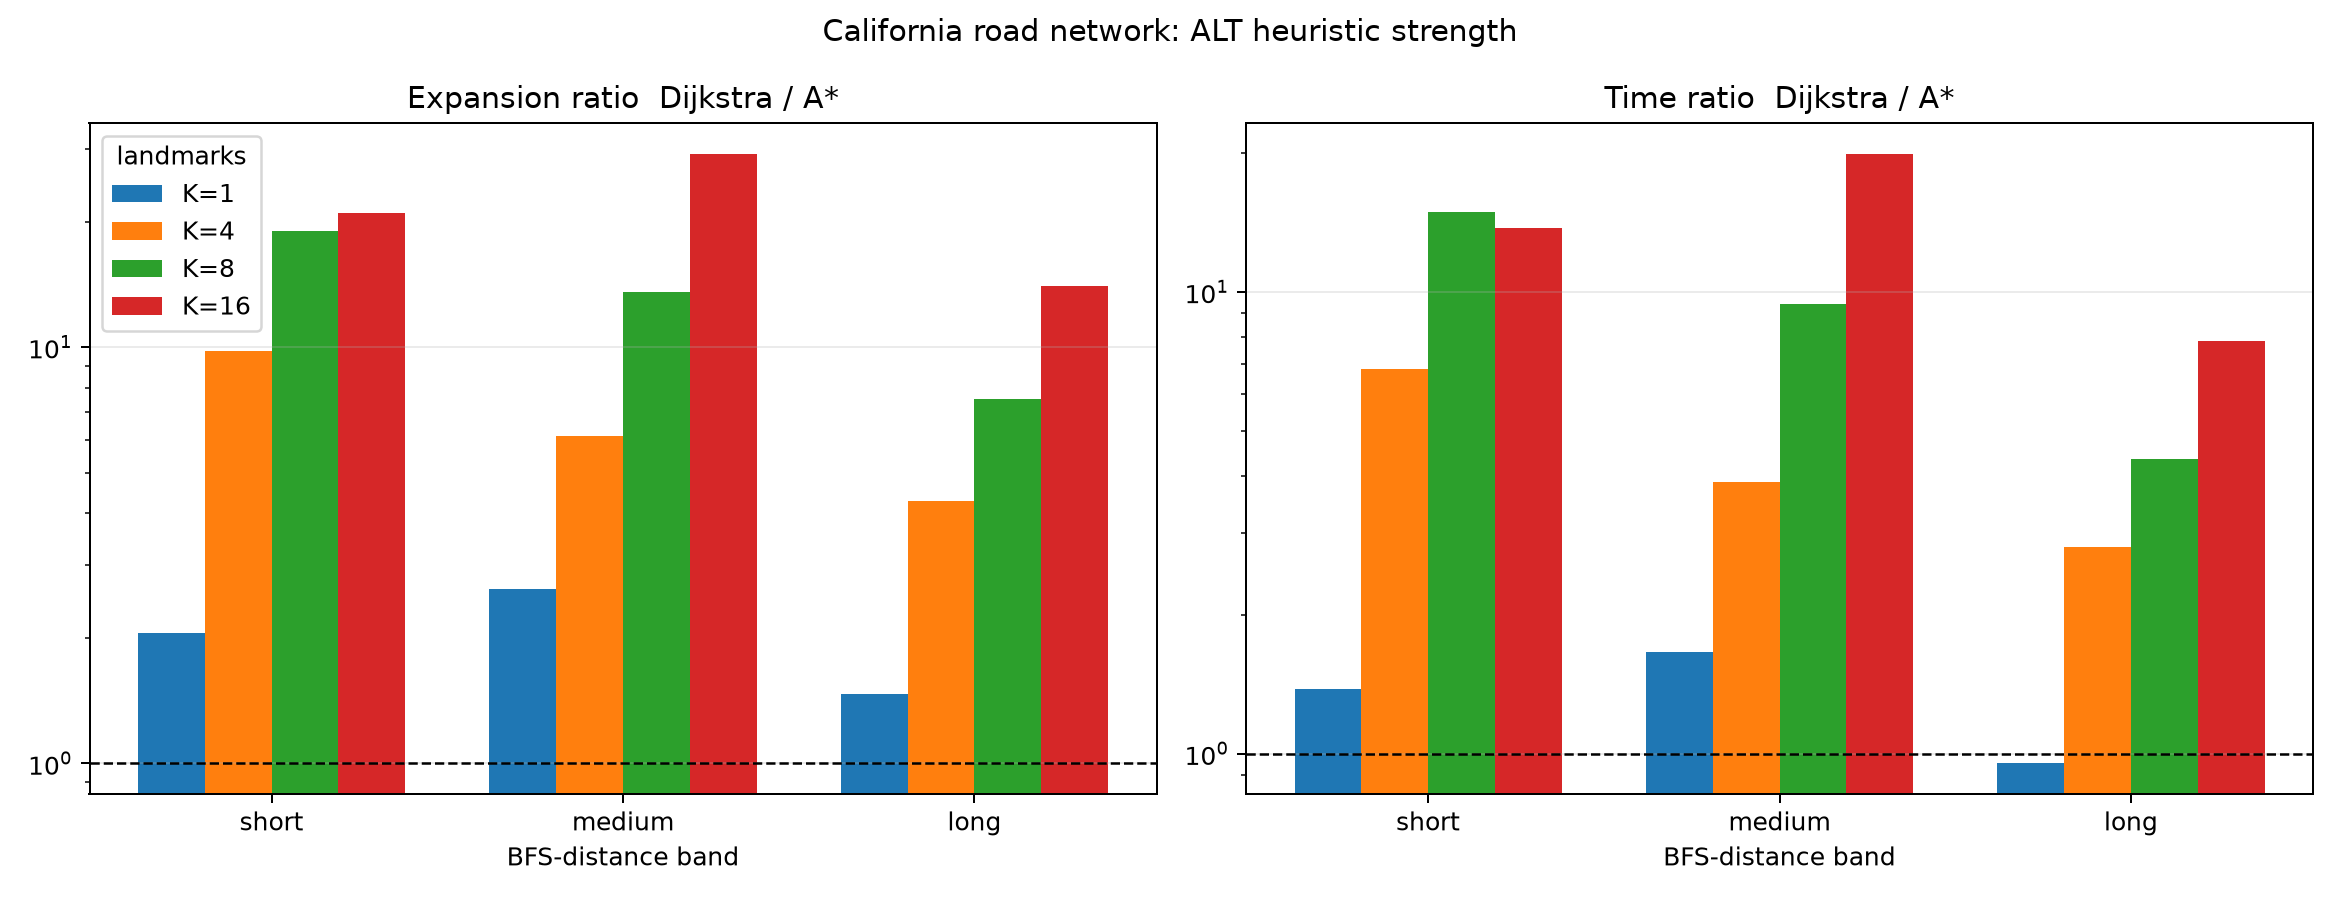
\includegraphics[width=\textwidth]{../figures/real_ratios_by_band_k.png}
    \end{column}
  \end{columns}
  \vspace{0.4em}
  \centering
  \small More landmarks keep tightening the bound; no plateau at 8 on this graph.
\end{frame}

\begin{frame}{Why time saving is smaller than expansion saving}
  \begin{columns}[T,onlytextwidth]
    \begin{column}{0.52\textwidth}
      \centering
      \small
      \begin{tabular}{lccc}
        \toprule
        family & Dijkstra & A* & ratio\\
               & ns/exp & ns/exp & \\
        \midrule
        open & 142 & 288 & 2.03x\\
        random & 157 & 254 & 1.62x\\
        clustered & 127 & 245 & 1.93x\\
        rooms & 146 & 270 & 1.85x\\
        maze & 65 & 79 & 1.21x\\
        \bottomrule
      \end{tabular}

      \vspace{0.6em}
      \footnotesize Real graph: Dijkstra 235 ns/exp; ALT K=8 373 ns (1.59x);
      K=16 394 ns (1.68x).
    \end{column}
    \begin{column}{0.46\textwidth}
      \centering
      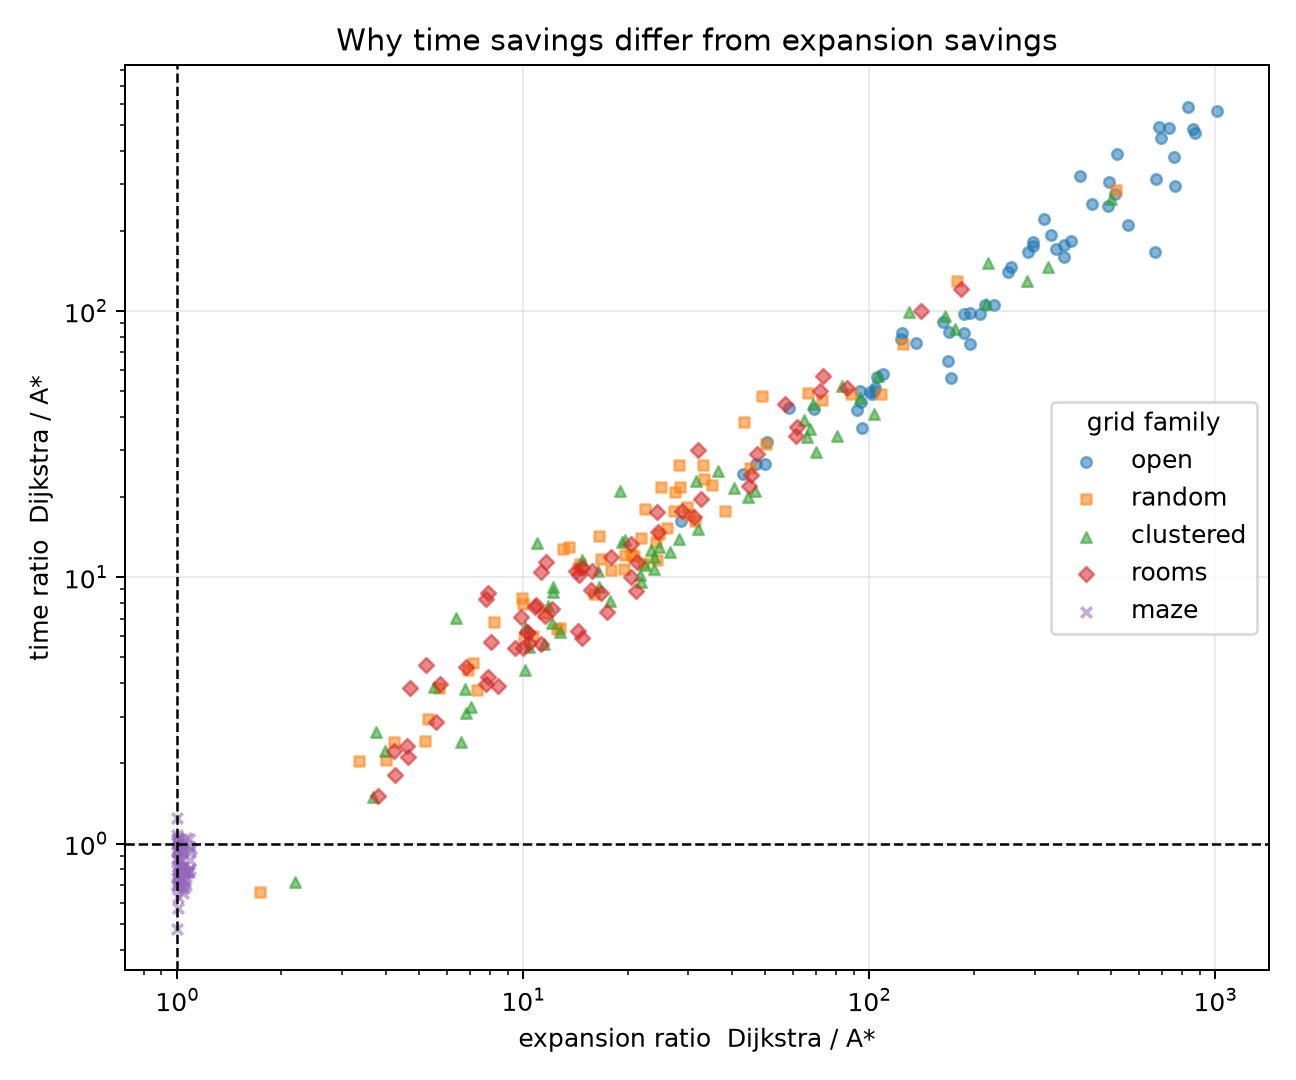
\includegraphics[width=\textwidth]{../figures/grid_time_vs_expansion.png}
    \end{column}
  \end{columns}
  \vspace{0.4em}
  \centering
  \textbf{The rule:} time is saved only when the expansion reduction pays for
  the more expensive expansion.
\end{frame}

\begin{frame}{Tie-breaking: a tail-risk decision}
  \begin{columns}[T,onlytextwidth]
    \begin{column}{0.47\textwidth}
      \small
      \setlength{\tabcolsep}{3pt}
      \begin{tabular}{lccc}
        \toprule
        family & median & node\_id worse & worst\\
               & ratio & queries & ratio\\
        \midrule
        open & 1.00 & 45\% & 285.7x\\
        random & 1.10 & 63\% & 51.5x\\
        clustered & 1.17 & 68\% & 92.6x\\
        rooms & 1.02 & 58\% & 17.8x\\
        maze & 1.00 & 2\% & 1.01x\\
        road (ALT K=8) & 1.14 & 90\% & 2.39x\\
        \bottomrule
      \end{tabular}

      \vspace{0.5em}
      Ratio = node\_id expansions / larger\_g expansions.\\
      On open, \texttt{larger\_g} never expanded more; it removes the
      catastrophic tail.  On the road graph, node\_id is worse on 27/30
      queries (expansion p$=4.4\times10^{-6}$).
    \end{column}
    \begin{column}{0.51\textwidth}
      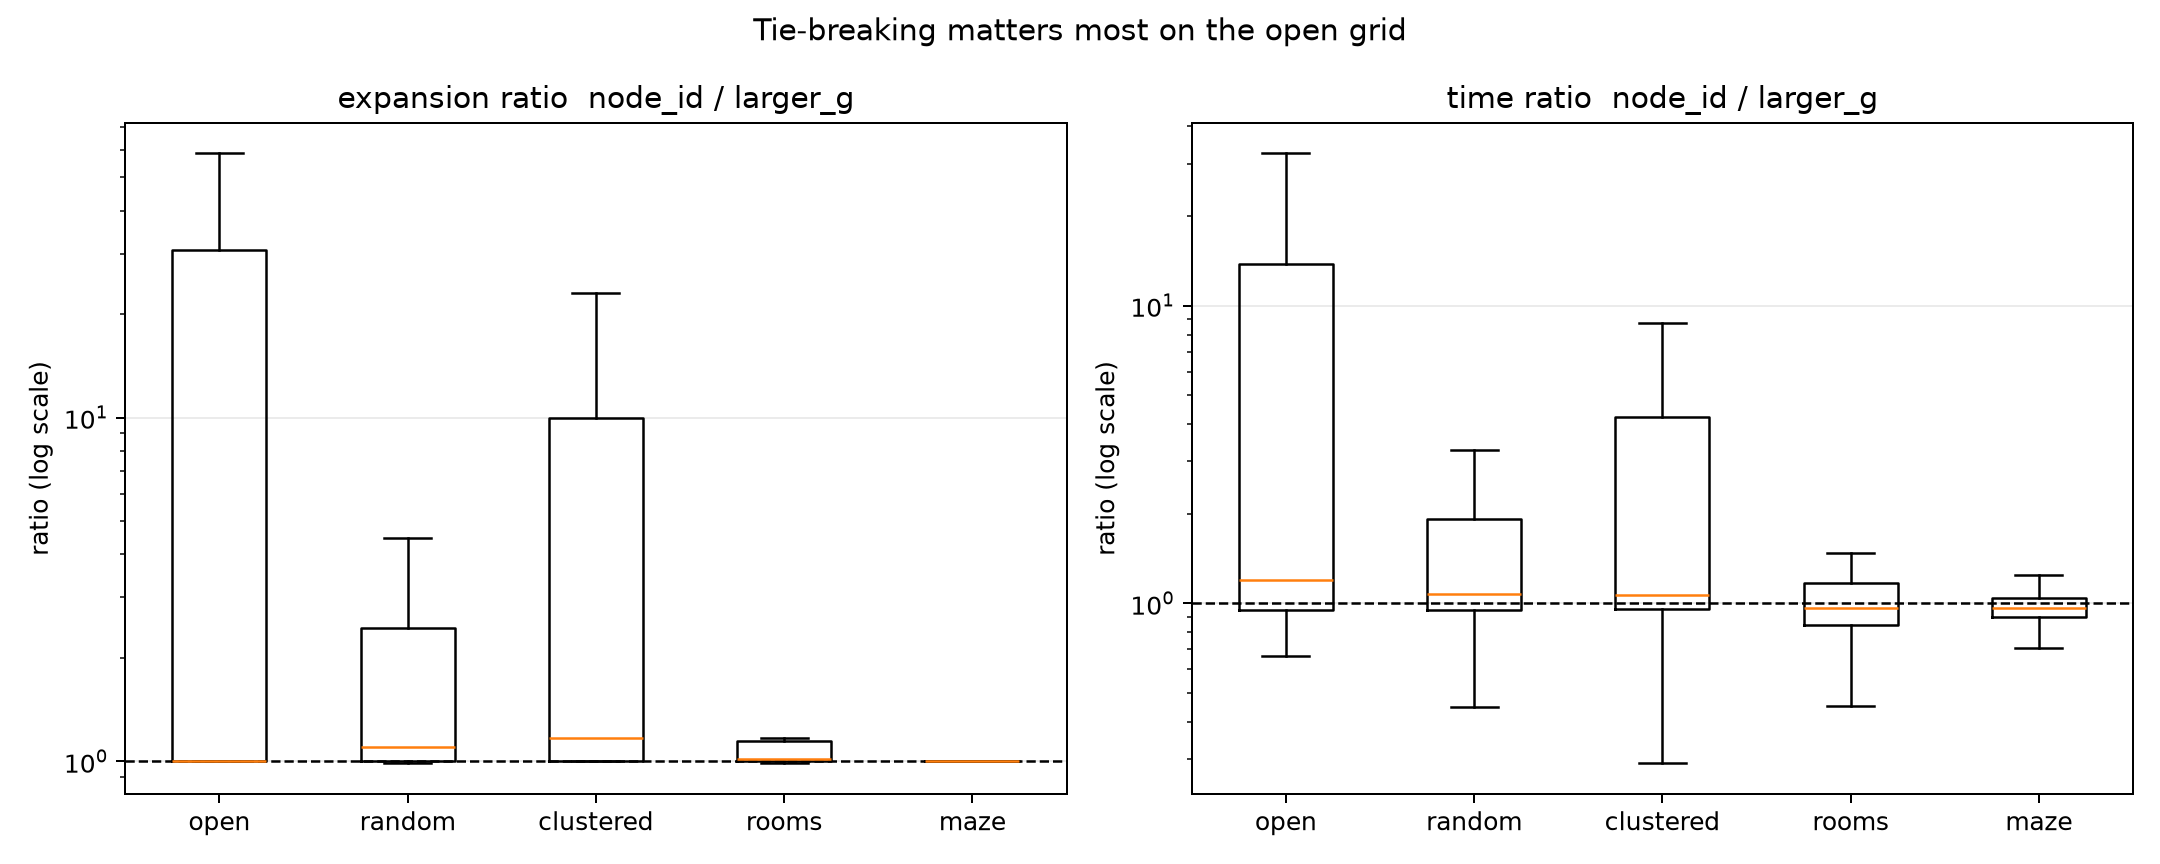
\includegraphics[width=\textwidth]{../figures/grid_tie_break.png}
    \end{column}
  \end{columns}
\end{frame}


\begin{frame}{What makes a heuristic informative?}
  \begin{columns}[T,onlytextwidth]
    \begin{column}{0.47\textwidth}
      \small
      \begin{tabular}{lccc}
        \toprule
        family & $h$ corr. & norm. MAE & time ratio\\
        \midrule
        open & 1.00 & 0.00 & 105.7x\\
        random & 1.00 & 0.02 & 12.8x\\
        clustered & 0.99 & 0.04 & 12.8x\\
        rooms & 0.99 & 0.06 & 8.7x\\
        maze & 0.42 & 0.97 & 0.81x\\
        \bottomrule
      \end{tabular}

      \vspace{0.5em}
      \footnotesize Pooled Spearman: $+0.78$ for $h$-distance correlation,
      $-0.81$ for normalised MAE.  A one-feature model has $R^2=0.55$.

      \vspace{0.4em}
      Admissibility is not enough: the heuristic must be
      \emph{informative} about the actual remaining distance.
    \end{column}
    \begin{column}{0.51\textwidth}
      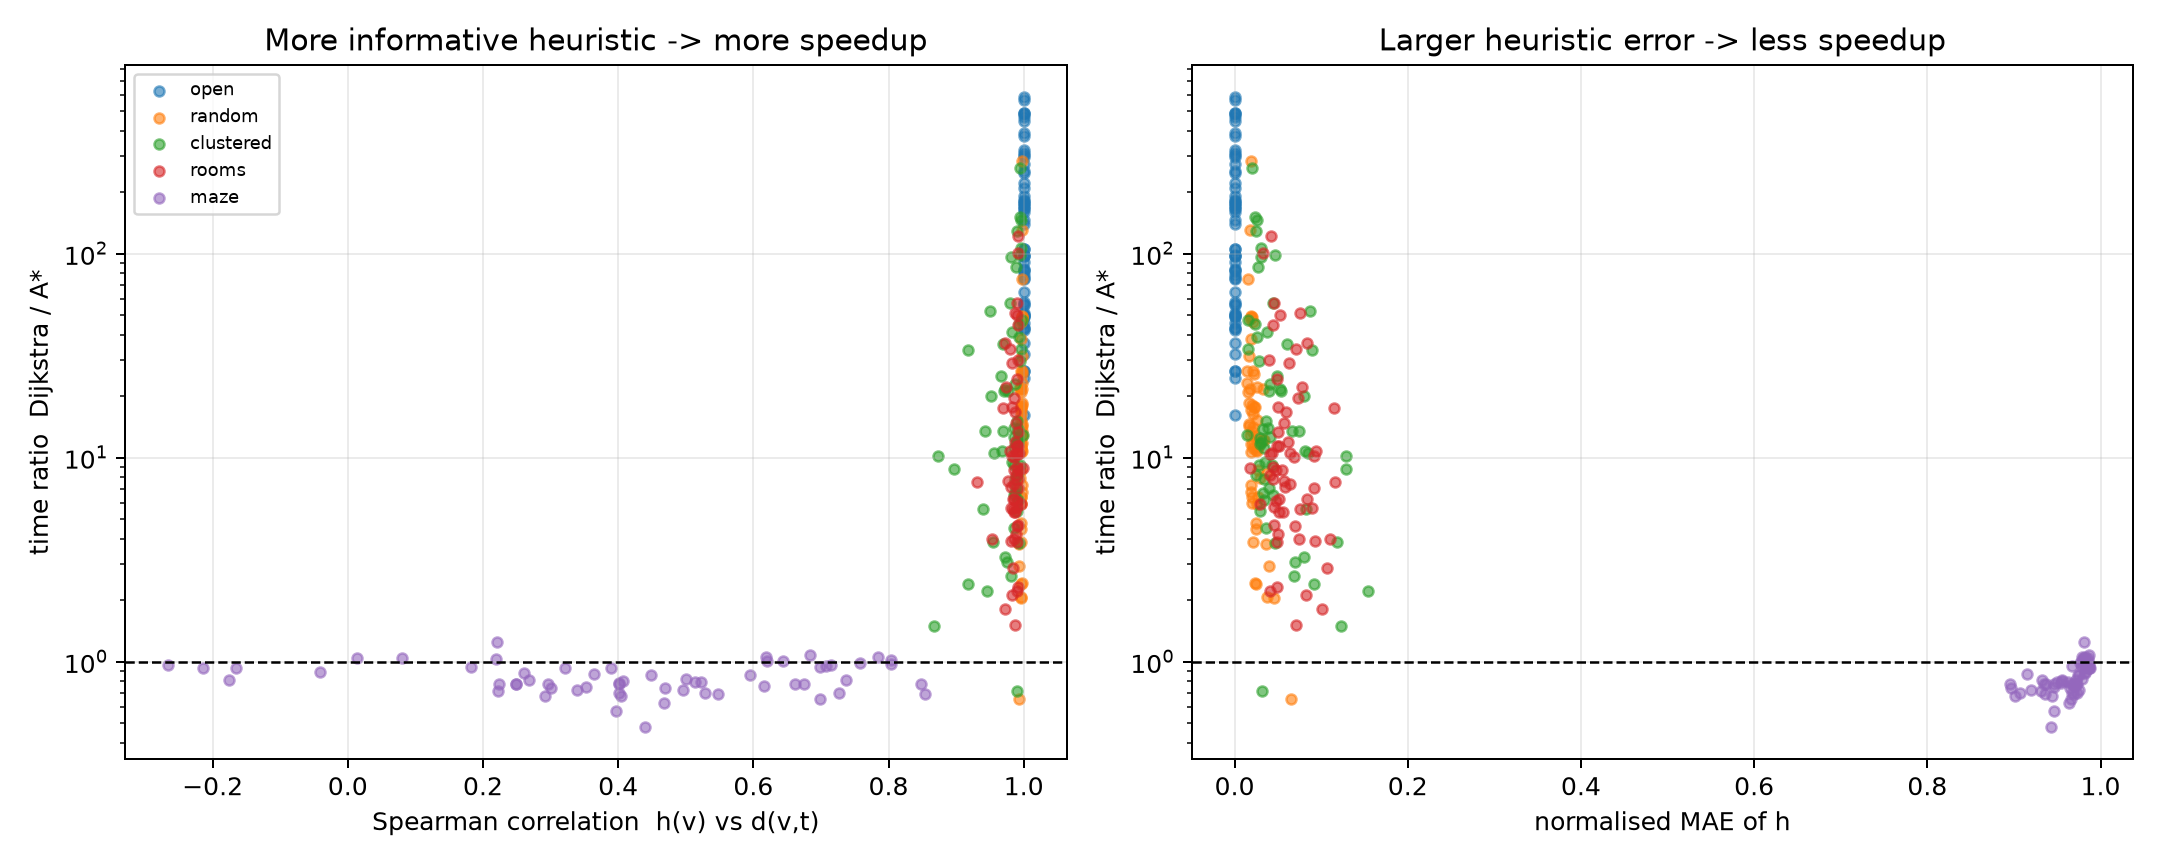
\includegraphics[width=\textwidth]{../figures/novelty_heuristic_speedup.png}
    \end{column}
  \end{columns}
\end{frame}

\begin{frame}{Weighted A*: price of optimality}
  \begin{columns}[T,onlytextwidth]
    \begin{column}{0.46\textwidth}
      \small
      \begin{tabular}{llcc}
        \toprule
        workload & $\epsilon$ & speed & cost\\
        \midrule
        random & 1.10 & 20.1x & 1.018\\
        random & 1.25 & 38.2x & 1.055\\
        rooms & 1.25 & 24.8x & 1.031\\
        clustered & 1.50 & 26.5x & 1.050\\
        maze & 50 & 1.10x & 1.000\\
        road & 1.00 & 7.4x & 1.000\\
        road & 1.10 & 8.8x & 1.014\\
        road, reopen & 1.10 & 5.4x & 1.011\\
        \bottomrule
      \end{tabular}

      \vspace{0.5em}
      \footnotesize $f=g+\epsilon h$, closed list except the last row.  All
      five grid families and the 30 road queries.  Speed is
      Dijkstra/weighted A*.  Maze and open grid are controls: their unique or
      exact paths keep cost at 1.00.
    \end{column}
    \begin{column}{0.52\textwidth}
      \small
      \textbf{Weak heuristic:} the first few percent of path cost buy a large
      amount of search.  Random obstacles move from 12.8x to 20.1x for 1.8\%
      median cost.

      \vspace{0.6em}
      \textbf{Strong heuristic:} on the road graph there is little to gain.
      The closed list improves 7.4x to 8.8x at 1.4\% cost; reopening falls to
      5.4x because reheapifying settled vertices costs more than the shorter
      search saves.

      \vspace{0.6em}
      \textbf{Rule:} weight when the heuristic is weak, keep
      $\epsilon\approx1.1$--$1.25$ if quality matters, and prefer a closed
      list.
    \end{column}
  \end{columns}
\end{frame}

\begin{frame}{Weighted A*: cost versus speed}
  \centering
  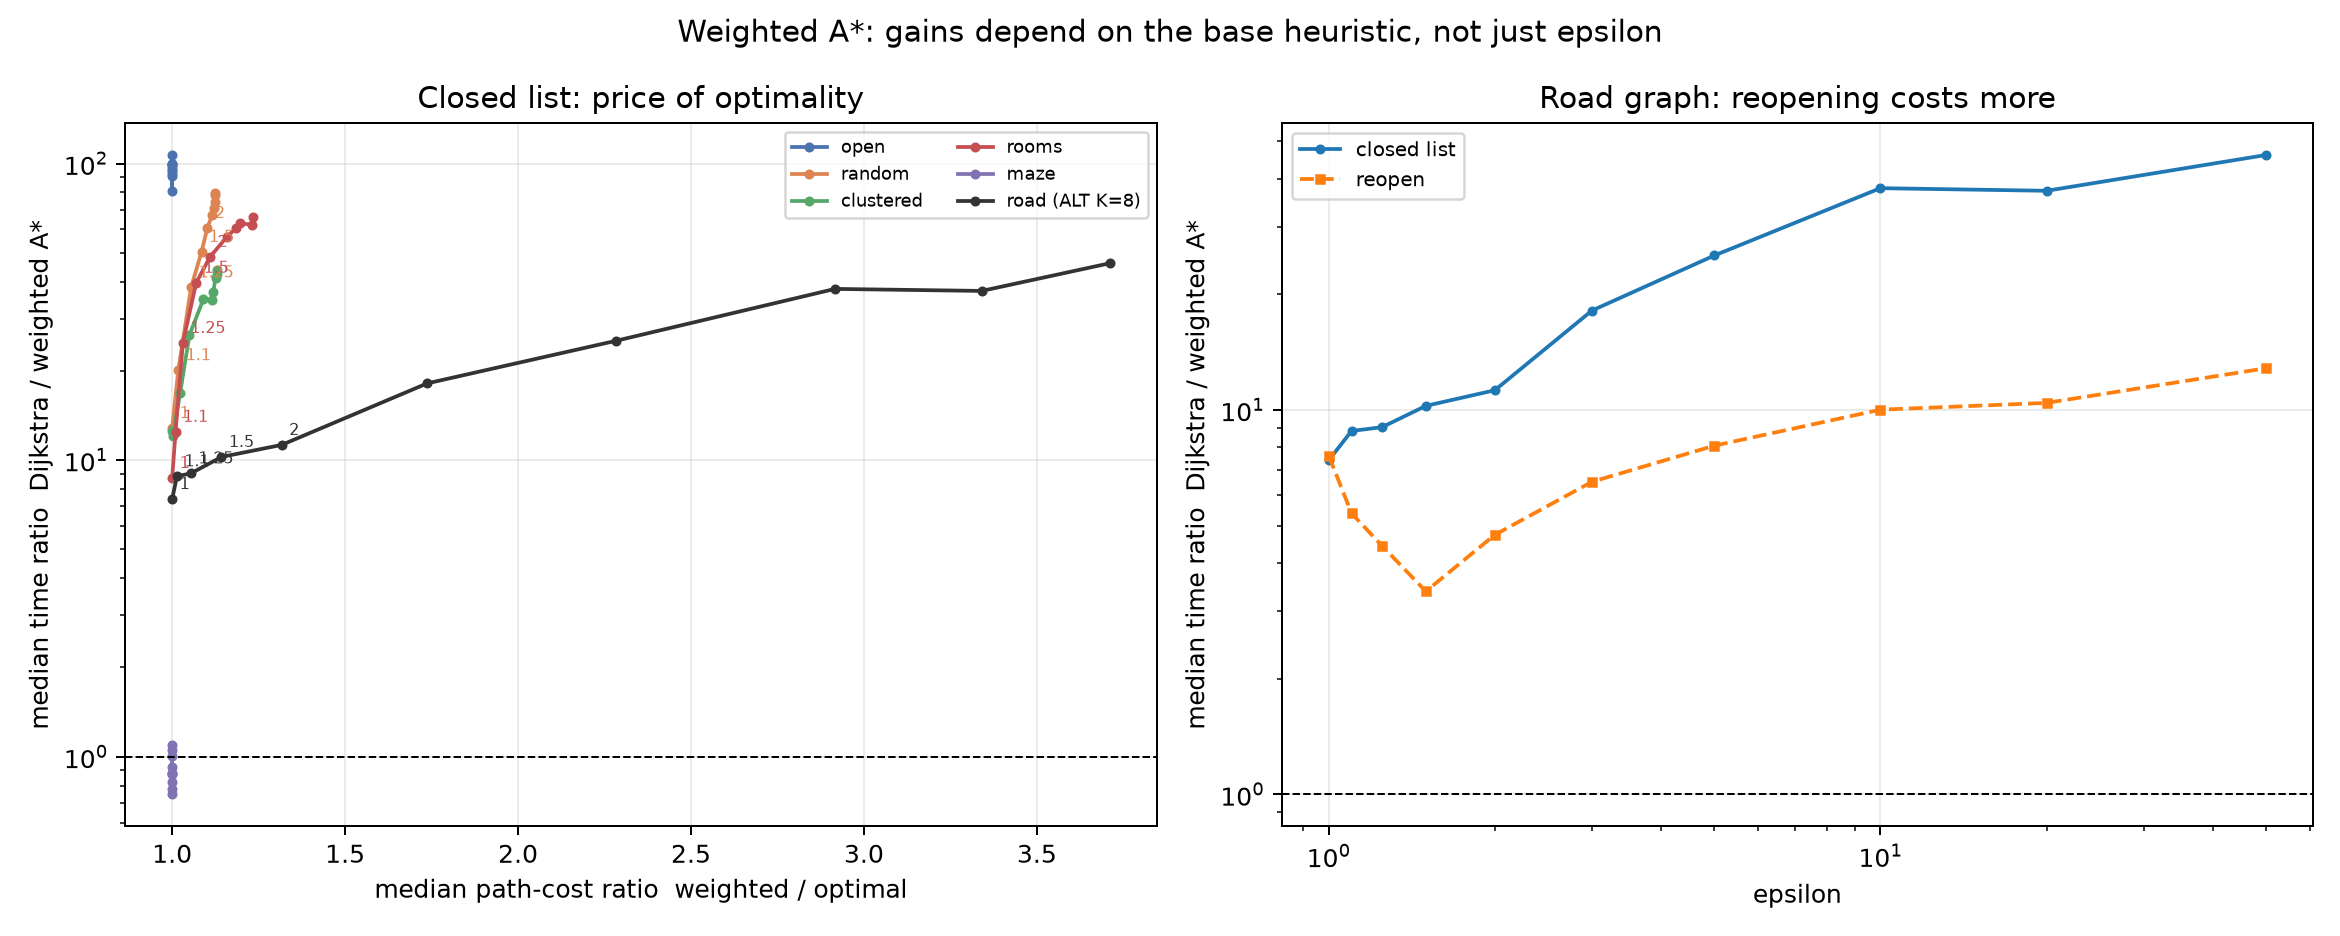
\includegraphics[width=\textwidth]{../figures/weighted_pareto.png}
  \vspace{0.3em}

  \footnotesize Left: closed-list frontier; points at cost 1.00 are the open
  grid and perfect maze, where there is no alternative path to trade.  Right:
  on the road graph the closed list is faster at every $\epsilon>1$, while
  reopening churns the heap for no useful gain.
\end{frame}


\begin{frame}{Does A* still win with 16 threads?}
  \begin{columns}[T,onlytextwidth]
    \begin{column}{0.43\textwidth}
      \small
      \begin{tabular}{rccc}
        \toprule
        threads & batch & speedup & efficiency\\
        \midrule
        1 & 44.39 s & 1.00x & 1.00\\
        2 & 21.48 s & 2.07x & 1.03\\
        4 & 10.11 s & 4.39x & 1.10\\
        8 & 6.27 s & 7.08x & 0.89\\
        16 & 4.56 s & \textbf{9.73x} & 0.61\\
        \bottomrule
      \end{tabular}

      \vspace{0.5em}
      \footnotesize Five $1024^2$ grids + 30 road queries, 3 repeats.  Each task
      runs Dijkstra and A* on the same query; thread-local scratch and
      heuristic.  A* advantage remains: median Dijkstra/A* ratio 14.8x at one
      thread, 17.9x at 16.  Maze stays below parity.
    \end{column}
    \begin{column}{0.55\textwidth}
      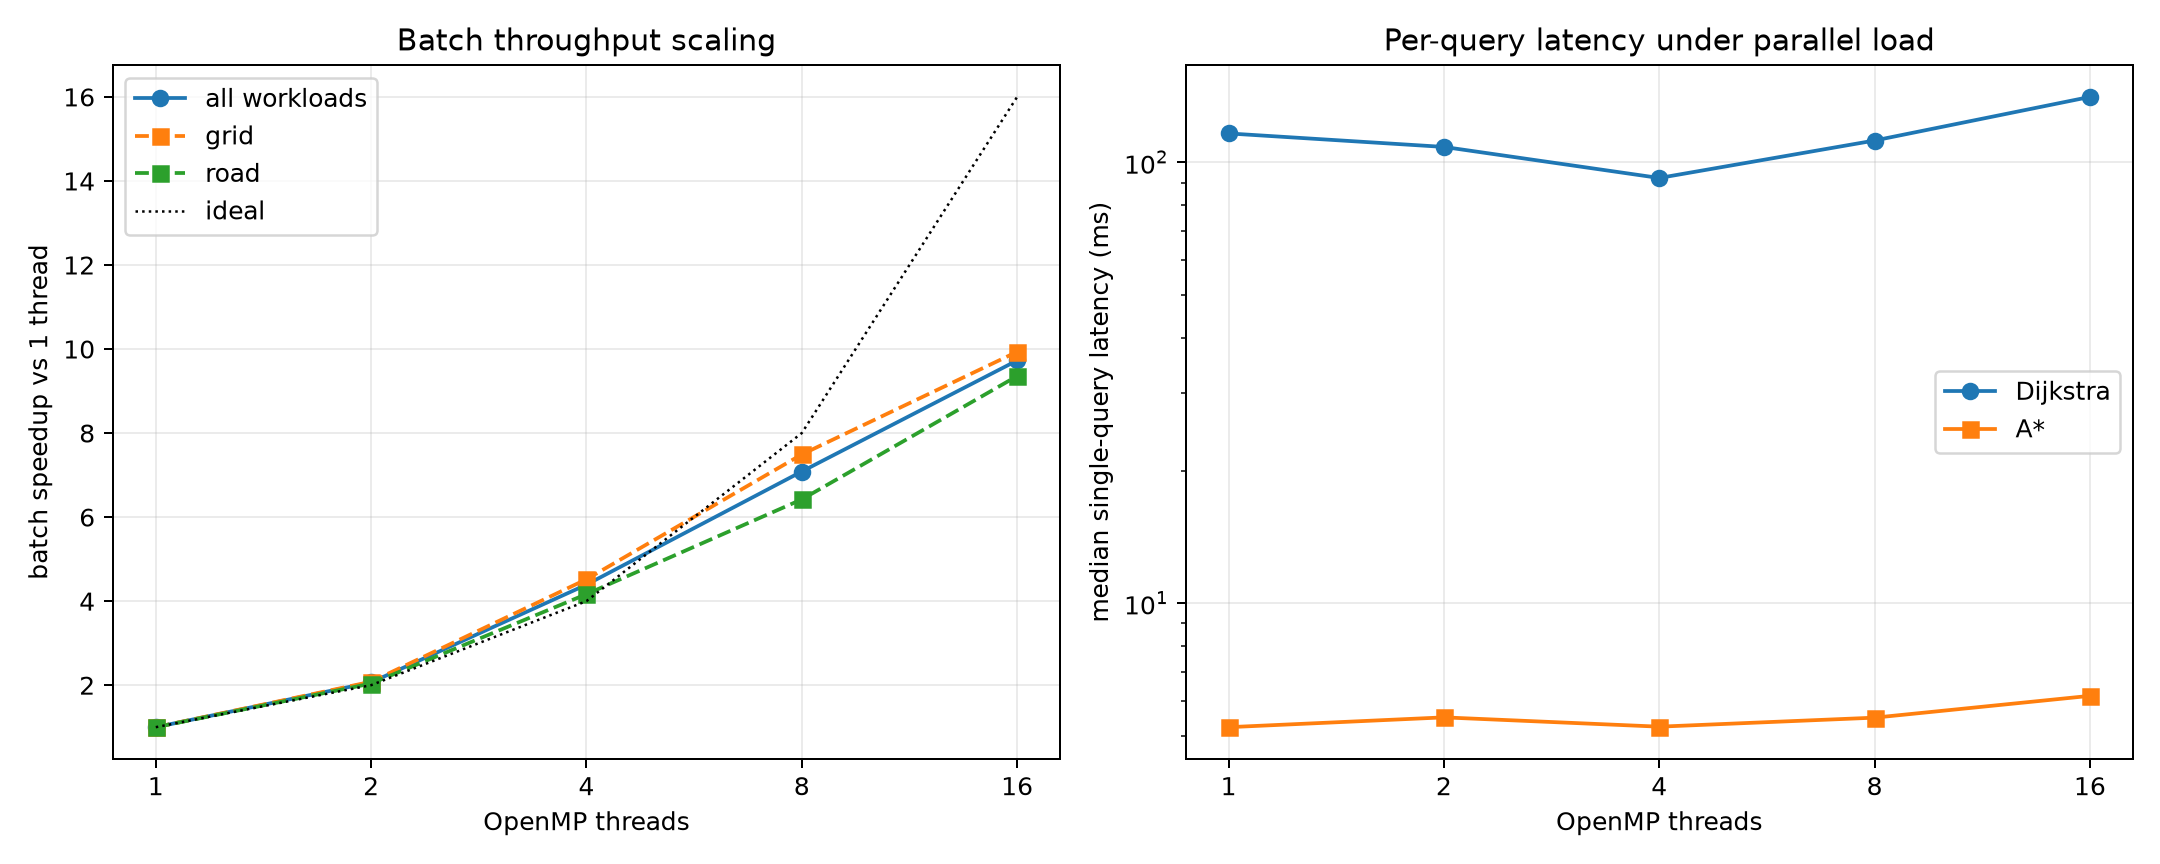
\includegraphics[width=\textwidth]{../figures/omp_scaling.png}
    \end{column}
  \end{columns}
  \vspace{0.3em}
  \centering
  \footnotesize Throughput gain, not single-query speedup.
\end{frame}

\begin{frame}{What the data rejected}
  \begin{itemize}
    \item \textbf{H5:} long queries do not always benefit more.  Open grid:
      long 156x vs short 83x time; random grid: long 11.5x vs short 14.4x.
    \item \textbf{H6 (diminishing returns):} K=16 is still better than K=8 on
      paired real queries (21\% time, 25\% expansions, p$<$1e-4).
    \item \textbf{H7 (median tie-break):} grid median is exactly 1.00 on the
      open grid, although 45\% of queries are worse with \texttt{node\_id}, up
      to 286x.  On the road graph, node\_id is worse on 27/30 queries (median
      1.14x, worst 2.39x).
    \item \textbf{The headline negative result:} in the maze, A* is 24\% slower
      even though its distances are correct.
  \end{itemize}
  \vspace{0.7em}
  \begin{block}{Interpretation}
    A null or negative result is still a result: guidance only pays when it
    changes the explored region, not merely when it is admissible.
  \end{block}
\end{frame}

\begin{frame}{Robustness: host performance mode}
  \centering
  \small
  \begin{tabular}{lccccc}
    \toprule
    workload & queries & Dijkstra speed-up & A* speed-up & ratio change & 95\% CI\\
             &         & (low/high mode)   & (low/high mode) & (high/low) & \\
    \midrule
    grid, sizes 128/512 & 150 & 2.24x & 2.23x & 1.011 & 0.994--1.028\\
    road, ALT K=8       & 30  & 2.26x & 2.23x & 0.993 & 0.967--1.020\\
    \bottomrule
  \end{tabular}

  \vspace{1.1em}
  \begin{columns}[T,onlytextwidth]
    \begin{column}{0.48\textwidth}
      \begin{block}{Matched subset}
        \footnotesize
        Same graphs, queries, seeds, bands and repeats as the frozen run.
        Expansions and distances are identical in both modes; only wall-clock
        time changes.
      \end{block}
    \end{column}
    \begin{column}{0.48\textwidth}
      \begin{block}{Result}
        \footnotesize
        The higher mode makes both algorithms $\approx$2.24x faster and leaves
        the A* ranking unchanged.  The maze loss persists; only absolute
        nanoseconds are mode-specific.
      \end{block}
    \end{column}
  \end{columns}

  \vspace{0.5em}
  \footnotesize
  No family changes significantly except open grid (ratio 0.954, $p=0.058$),
  where A* runs in only 17--133 $\mu$s per query.
\end{frame}

\begin{frame}{Threats to validity}
  \begin{columns}[T,onlytextwidth]
    \begin{column}{0.50\textwidth}
      \begin{itemize}
        \item one real graph; road network, not a sample of all real graphs
        \item unit hop weights; no travel times in SNAP
        \item symmetrised roads; one-way streets not modelled
        \item synthetic grid families are controls, not real maps
        \item one machine, one heap implementation
      \end{itemize}
    \end{column}
    \begin{column}{0.47\textwidth}
      \begin{itemize}
        \item medians and IQRs, bootstrap CIs, paired Wilcoxon
        \item within-query time CV 7--10\%
        \item all 3,600 runs match BFS; no timeouts
        \item raw CSV and seeds are kept
        \item protocol frozen before the main run
      \end{itemize}
    \end{column}
  \end{columns}
  \vspace{0.6em}
  \centering
  \small The constants are implementation- and machine-specific; the direction
  and the mechanism are the transferable result.
\end{frame}

\begin{frame}{Final answer}
  \begin{block}{When does A* save work?}
    When the heuristic is informative about the \emph{actual} remaining path,
    and the reduction in expanded vertices is large enough to pay for the
    more expensive expansion.
  \end{block}
  \begin{itemize}
    \item \textbf{Open grid:} yes, spectacularly (106x time, 222x expansions).
    \item \textbf{Random/clustered/rooms:} yes, but 9--13x time, not 100x.
    \item \textbf{Maze:} no; 24\% slower, because Manhattan cannot see walls.
    \item \textbf{Road network:} yes; ALT K=8 7.6x, K=16 13.5x.
    \item \textbf{Weighted A*:} a closed list buys 20x at 1.8\% cost on random
      obstacles; on the road graph reopening costs more than it saves.
    \item \textbf{Tie-break:} \texttt{larger\_g} is the safe default;
      \texttt{node\_id} is worse on 27/30 road queries.
    \item \textbf{Practical rule:} measure expansions and cost per expansion;
      do not assume the heuristic is free.
  \end{itemize}
\end{frame}

\begin{frame}{Reproduce}
  \small
  \begin{block}{Build and test}
    \texttt{cmake -S . -B build -DCMAKE\_BUILD\_TYPE=Release}\\
    \texttt{cmake --build build -j}\\
    \texttt{./build/test\_core}
  \end{block}
  \begin{block}{Full frozen run}
    \texttt{./scripts/run\_experiments.sh}
  \end{block}
  \begin{block}{Artifacts}
    \texttt{HYPOTHESES.md}, \texttt{PROTOCOL.md}, \texttt{RESULTS.md},\\
    \texttt{results/grid.csv}, \texttt{results/real.csv},
    \texttt{results/analysis.md}, \texttt{figures/}
  \end{block}
  \vspace{0.6em}
  \centering
  \Large Questions?
\end{frame}

\end{document}
